\documentclass[12pt,a4paper]{article}

\usepackage{ctex}

\usepackage{geometry}%用于设置上下左右页边距
\usepackage{amsmath,paralist,enumerate,booktabs,
multirow,graphicx,subfig,setspace,listings,lastpage}
%amsmath:数学公式
%paralist,enumerate:自定义项目符号
%booktabs:三线图,论文常用的表格风格
%multirow:复杂表格
%graphicx,float: 插入图片
%subfig:并排排版图片、竖向排版图片
%setspace:设置行间距等功能
\setlength{\parindent}{2em}%正文首行缩进两个汉字

\usepackage{hyperref}
\hypersetup{
    hidelinks
}

\usepackage{fancyhdr}
\setlength{\headheight}{14.5pt} % 设置页眉高度
\addtolength{\topmargin}{-2.5pt} % 设置页眉与顶部的距离

\pagestyle{fancy}
%分别是右页眉、左页眉、中页脚、右页脚
\rhead{实验B01 参考文献的检索和管理}
\lhead{基础物理实验\uppercase\expandafter{\romannumeral2}实验报告}
\cfoot{Page \thepage/\pageref{LastPage}}  %当前页\总页数
\rfoot{\today}

\renewcommand{\headrulewidth}{0.4pt}
\renewcommand{\theenumi}{(\arabic{enumi})}

%%%%%%%%%%%%%%%%%%%%%%%%%%%%%%%%%%%%%%%%%%%%%%%%%%%%%%%%%%
%%%%%%%%%%%%%%%%%%%%%%%%%正文开始%%%%%%%%%%%%%%%%%%%%%%%%%%
%%%%%%%%%%%%%%%%%%%%%%%%%%%%%%%%%%%%%%%%%%%%%%%%%%%%%%%%%%

\begin{document}

%%begin-------------------标题与信息-----------------------%%

%%标题
\begin{center}
\LARGE\textbf{实验B01 参考文献的检索和管理}
\end{center}

%%信息
\begin{doublespacing}
	%doublespacing:手动两倍行距
	\centering
	\begin{tabular}{p{6.5cm}p{6.5cm}}
	 & \\
	 实验人姓名、学号: & 合作者姓名、学号:无\\
	 {时间:2024年9月20日星期五上午} & {实验地点:南校区陆祐堂104}\\
	 {室温:26$^{\circ}$C} & 相对湿度:59\%
	
	\end{tabular}
\end{doublespacing}

%%end-------------------标题与信息-----------------------%%


\subsection*{【实验目的】}
%*表示不带上小节本身应有的1.1,下面的subsubsection*也是一样
%%自定义项目符号之(1)(2)(3)
	\begin{enumerate}[(1)]
		\item 学习利用NoteExpress(或Endnote)软件检索和管理科技文献。
		\item 学习利用NoteExpress(或Endnote)与Microsoft Word配合写作的方法。
	\end{enumerate}

\subsection*{【仪器用具】}
%%一般表格
%所有表格都可以通过Excel2LaTex加载项,在excel中转换成以下一串代码。需要琢磨的是调节一些细节的方法。
% Table generated by Excel2LaTeX from sheet 'Sheet1'
	\begin{table}[htbp]
	  \centering
	    \begin{tabular}{cccp{20em}}
	    \toprule
	    编号    & 仪器用具名称 & 数量    & 主要参数(型号,测量范围,测量精度等) \\
	    \midrule
	    1     & 计算机 & 1     &  \\
	    \bottomrule
	    \end{tabular}%
	  \label{tab:device}%
	\end{table}%

\subsection*{【实验原理】}

	\subsubsection*{1.参考文献的检索、管理、阅读和引用}
		参考文献的检索、管理、阅读和引用是学术研究工作的一项重要内容。按照
	最新颁布的国家标准GB/T 7714-2015《信息与文献 参考文献著录规则》中的定
	义,参考文献是指“为撰写或编辑论文和著作而引用的有关文献信息资源”\cite{bandyopadhyay_physics_2009},
	包括专著、期刊论文、学位论文、专利、技术标准、网页、音像资料等数十种类
	型。参考文献的质量是评价学术成果质量的一个重要指标。本科阶段的学生,有
	必要尽快掌握参考文献的检索、管理和正确引用方法。\cite{gonzalez-garcia_phenomenology_2008}
	在利用Microsoft Word 进行科技论文、学位论文和实验报告的写作时,如
	果文献较少,可以利用软件中“引用”菜单中的“插入引文”功能完成参考文献
	的引用和自动排序,但参考文献数量较大时,利用专业的参考文献管理软件可极
	大地提高工作效率和准确率。目前,常用的参考文献管理软件有许多种\cite{meloni_sterile_2010},如
	Endnote、NoteExpress、NoteFirst、Citavi、Mendeley、Zotero 等。这些软件各有特
	色,如支持哪种操作系统,是否有单机版和网络版,支持哪种浏览器\cite{tang_neutrino_2010},免费版还
	是收费版等,建议使用者根据自己的实际情况,选择其中至少一种软件并熟练掌
	握其使用方法。\cite{tang_requirements_2012}


	\subsubsection*{2.NoteExpress国产的文献管理软件}


\subsection*{【实验内容及步骤】}
	\subsubsection*{1.}



\subsection*{【数据处理及分析】}

	\subsubsection*{1.有机玻璃的导热系数$\lambda$和比热容c}

	\begin{table}[htbp]
	\centering
		\caption{有机玻璃实验结果}
		\vspace{1em}
	  	\resizebox{\textwidth}{20mm}%第一个大括号为宽度,第二个大括号为高度(60mm)可随机设置,调整到适合该表格的大小为止
		{ 
	    \begin{tabular}{ccccccc}
	    \toprule
	    时间$\tau/s$ & 温差热电势$V_t/mV$ & 中心面热电势$V_c/mV$ & 温度差$\Delta t/^{\circ}$C & 中心面温度$t_c^{\circ}$C & $\Delta V/mV$ & $a\tau/R^2$ \\
	    \midrule
	    120   & 0.109 & 0.023 & 2.72 & 20.57 & 0.005 & 0.115 \\
	    180   & 0.142 & 0.036 & 3.55 & 20.90 & 0.013 & 0.172 \\
	    240   & 0.162 & 0.053 & 4.05 & 21.32 & 0.017 & 0.230 \\
	    300   & 0.173 & 0.073 & 4.32 & 21.82 & 0.020 & 0.288 \\
	    360   & 0.180 & 0.095 & 4.50 & 22.37 & 0.022 & 0.346 \\
	    420   & 0.185 & 0.118 & 4.62 & 22.95 & 0.023 & 0.403 \\
	    480   & 0.188 & 0.141 & 4.70 & 23.52 & 0.023 & 0.460 \\
	    \bottomrule
	    \end{tabular}
		}
	  	\label{tab:data}
	\end{table}

	\paragraph{(1)求有机玻璃的导热系数$\lambda$和比热容c}
	
	\begin{table}[htbp]
		\centering
			\caption{表名}
			\vspace{1em}
			\resizebox{0.2\textwidth}{25.0mm}
			{
			\begin{tabular}{cc}
			\toprule
			x1 & x2 \\
			\midrule
			0.5 & 12.06 \\
			0.531 & 17.16 \\
			0.563 & 27.77 \\
			0.594 & 65.18 \\
			0.625 & 51.01 \\
			0.656 & 24 \\
			0.688 & 14.99 \\
			0.719 & 10.77 \\
			0.725 & 8.14 \\
			\bottomrule
			\end{tabular}
			}
			\label{tab:data2}
	\end{table}
	
%%%%%%%%%%%%%%%%%%%%%%%%%%%%%%%%%%%%%%%%%%%%%%
%%%%%%%%%%%%%%%%%图片的插入%%%%%%%%%%%%%%%%%%%%
%%%%%%%%%%%%%%%%%%%%%%%%%%%%%%%%%%%%%%%%%%%%%%

%% 单幅图插入
	% 图片的大小需要细细得调。需要掌握latex里面的长度单位和限制大小方法。
	\begin{figure}[htbp]
		\centering
		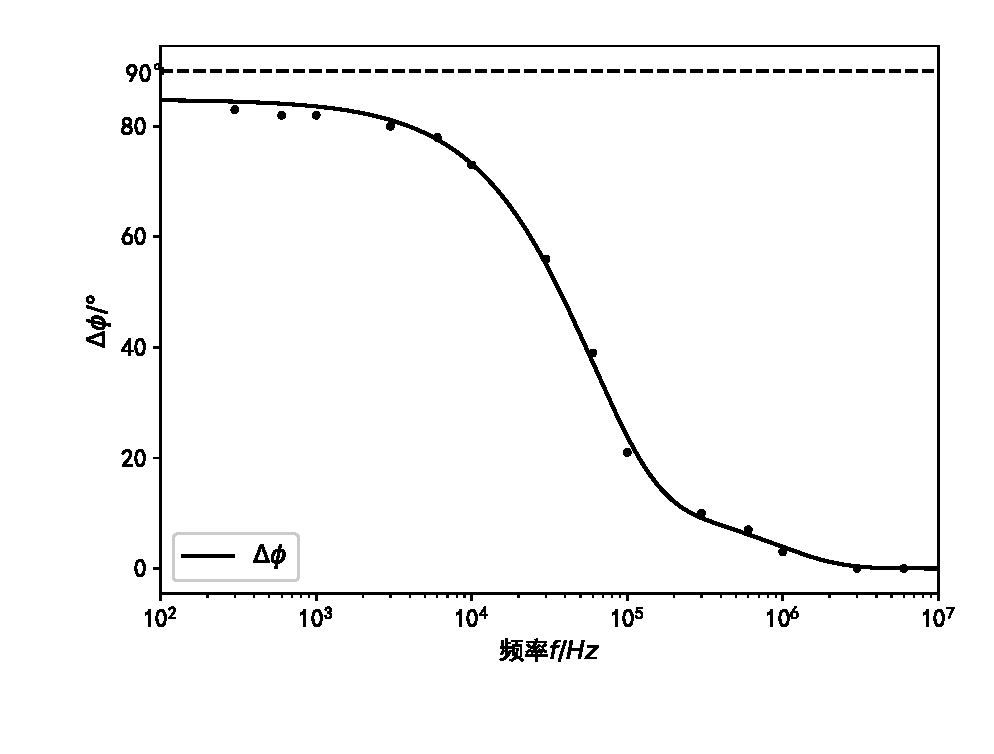
\includegraphics[width=\textwidth]{img//1.eps}
		\caption{相频特性曲线(矢量图)}
	\end{figure}

%% 两幅图并行排版,各有图题,还有一个总的图题
	% (1)注意正文中引用图片的方法,label可以打在minipage前面,也可以打在总图题的后面。
	% (2)需要调节图片大小,也可以调节位置。通过{minipage}后面的补充参数来调节位置。图片大小可以用高度来调以保证两个图高度一样。
	\begin{figure}[htbp]
		\centering
		\subfloat[相频特性曲线(位图)]{\label{fig:nogamma4}
		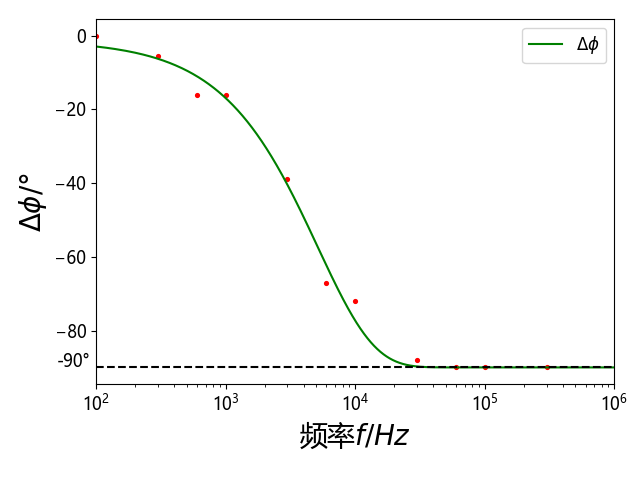
\includegraphics[width=0.4\textwidth]{img/3_1.png}%调节这里的图片宽度
		}%
		\subfloat[相频特性曲线]{\label{fig:withgamma4}
		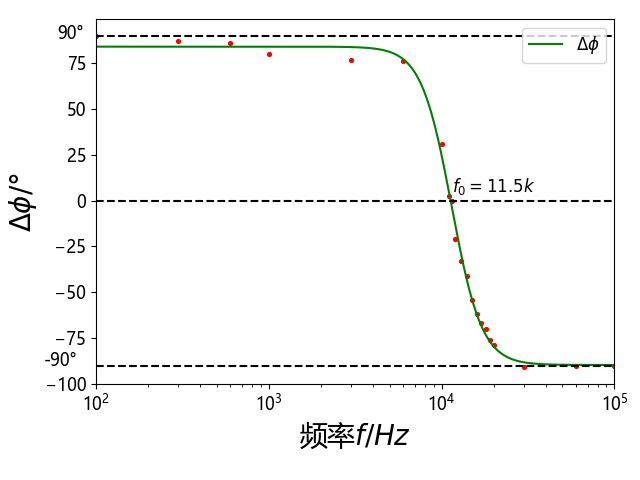
\includegraphics[width=0.4\textwidth]{img/3_2.png}%调节这里的图片宽度
		}%
		\caption{相频特性曲线}
		\label{fig:tcvi}
	\end{figure}

%%%%%%%%%%%%%%%%%%%%%%%%%%%%%%%%%%%%%%%
%%%%%%%%%%%%%%%插入公式%%%%%%%%%%%%%%%%%
%%%%%%%%%%%%%%%%%%%%%%%%%%%%%%%%%%%%%%%
\newpage
\paragraph*{公式的插入}


\subsection*{【思考题】}
	\subsubsection*{1.检索若干种参考文献管理软件的说明文件,对比它们的优缺点。}
	\subsubsection*{2.查阅帮助文件,实现参考文献的多人共享,网络与本地文献同步等其他功能。}

\newpage

% 参考文献
\bibliographystyle{plain}
\bibliography{reference}

	
\end{document}
